\chapter{Methodologie und Systementwurf }

In diesem Kapitel wird erklärt, wie das Projekt „LibraNova“  geplant und technisch umgesetzt wurde. Zuerst wird die Projektidee mithilfe von UML-Diagrammen dargestellt. Danach folgen die eingesetzten Technologien im Frontend und Backend sowie der Aufbau der Datenbank. Auch Themen wie Sicherheit, Entwicklungswerkzeuge und Softwaretests werden behandelt, um einen vollständigen Überblick über den Systementwurf zu geben.



\section{Entwurf und Konzeption}\index{Entwurf und Konzeption}

In der Softwareentwicklung spielen Entwurf und Konzeption eine zentrale Rolle. Diese Phase des Entwicklungsprozesses dient dazu, die Struktur und das Verhalten eines Systems frühzeitig zu planen, bevor mit der eigentlichen Implementierung begonnen wird. Ziel ist es, ein klares und verständliches Modell zu erstellen, das die Anforderungen und Abläufe der Anwendung abbildet. In diesem Abschnitt werden exemplarisch einige Diagrammtypen vorgestellt, die zur Modellierung des Projekts verwendet wurden.


\subsection{Einführung in UML}\index{Einführung in UML}

Die Unified Modeling Language (UML) ist ein wesentliches Werkzeug im Bereich Entwurf. UML ist eine standardisierte Modellierungssprache, die eine Vielzahl von Diagrammen bietet, um unterschiedliche Aspekte eines Systems darzustellen. Diese Diagramme helfen dabei, komplexe Systeme zu visualisieren, zu dokumentieren und zu kommunizieren \cite{UML:2023}. 

\subsection{Klassendiagramm}\index{Klassendiagramm}

Das unten stehenden Klassendiagramm \ref{fig:class_diagram} stellt die grundlegende Struktur der Anwendung dar und dient als Übersicht über die zentralen Klassen sowie deren Beziehungen untereinander. Es bildet sowohl die Domänenlogik (z.\,B. Bücher, Ausleihen, Rezensionen) als auch das Benutzer- und Kommunikationsmanagement (z.\,B. Kunden, Administratoren, Nachrichten) ab. \\ 
Die Benutzerklassen \texttt{Admin} und \texttt{Customer} erben von der abstrakten Oberklasse \texttt{User}, wodurch eine klare Trennung der Rollen und Verantwortlichkeiten ermöglicht wird. Die Klasse \texttt{Book} steht im Zentrum der Bibliotheksbereich und ist über Assoziationen mit \texttt{Checkout}, \texttt{Review}, \texttt{History} sowie mit den Benutzerklassen verbunden. Diese Assoziationen repräsentieren unter anderem ausgeliehene Bücher, verfasste Rezensionen oder Verwaltungsvorgänge.\\ 
Auch die Interaktionen zwischen Kunden und Administratoren über Nachrichten werden modelliert, ebenso wie die Historie vergangener Ausleihvorgänge. Das Diagramm stellt somit eine strukturierte Grundlage für die Implementierung dar und verdeutlicht die Zusammenhänge zwischen den einzelnen Komponenten der Anwendung.

\begin{figure}[H]
	\centering
	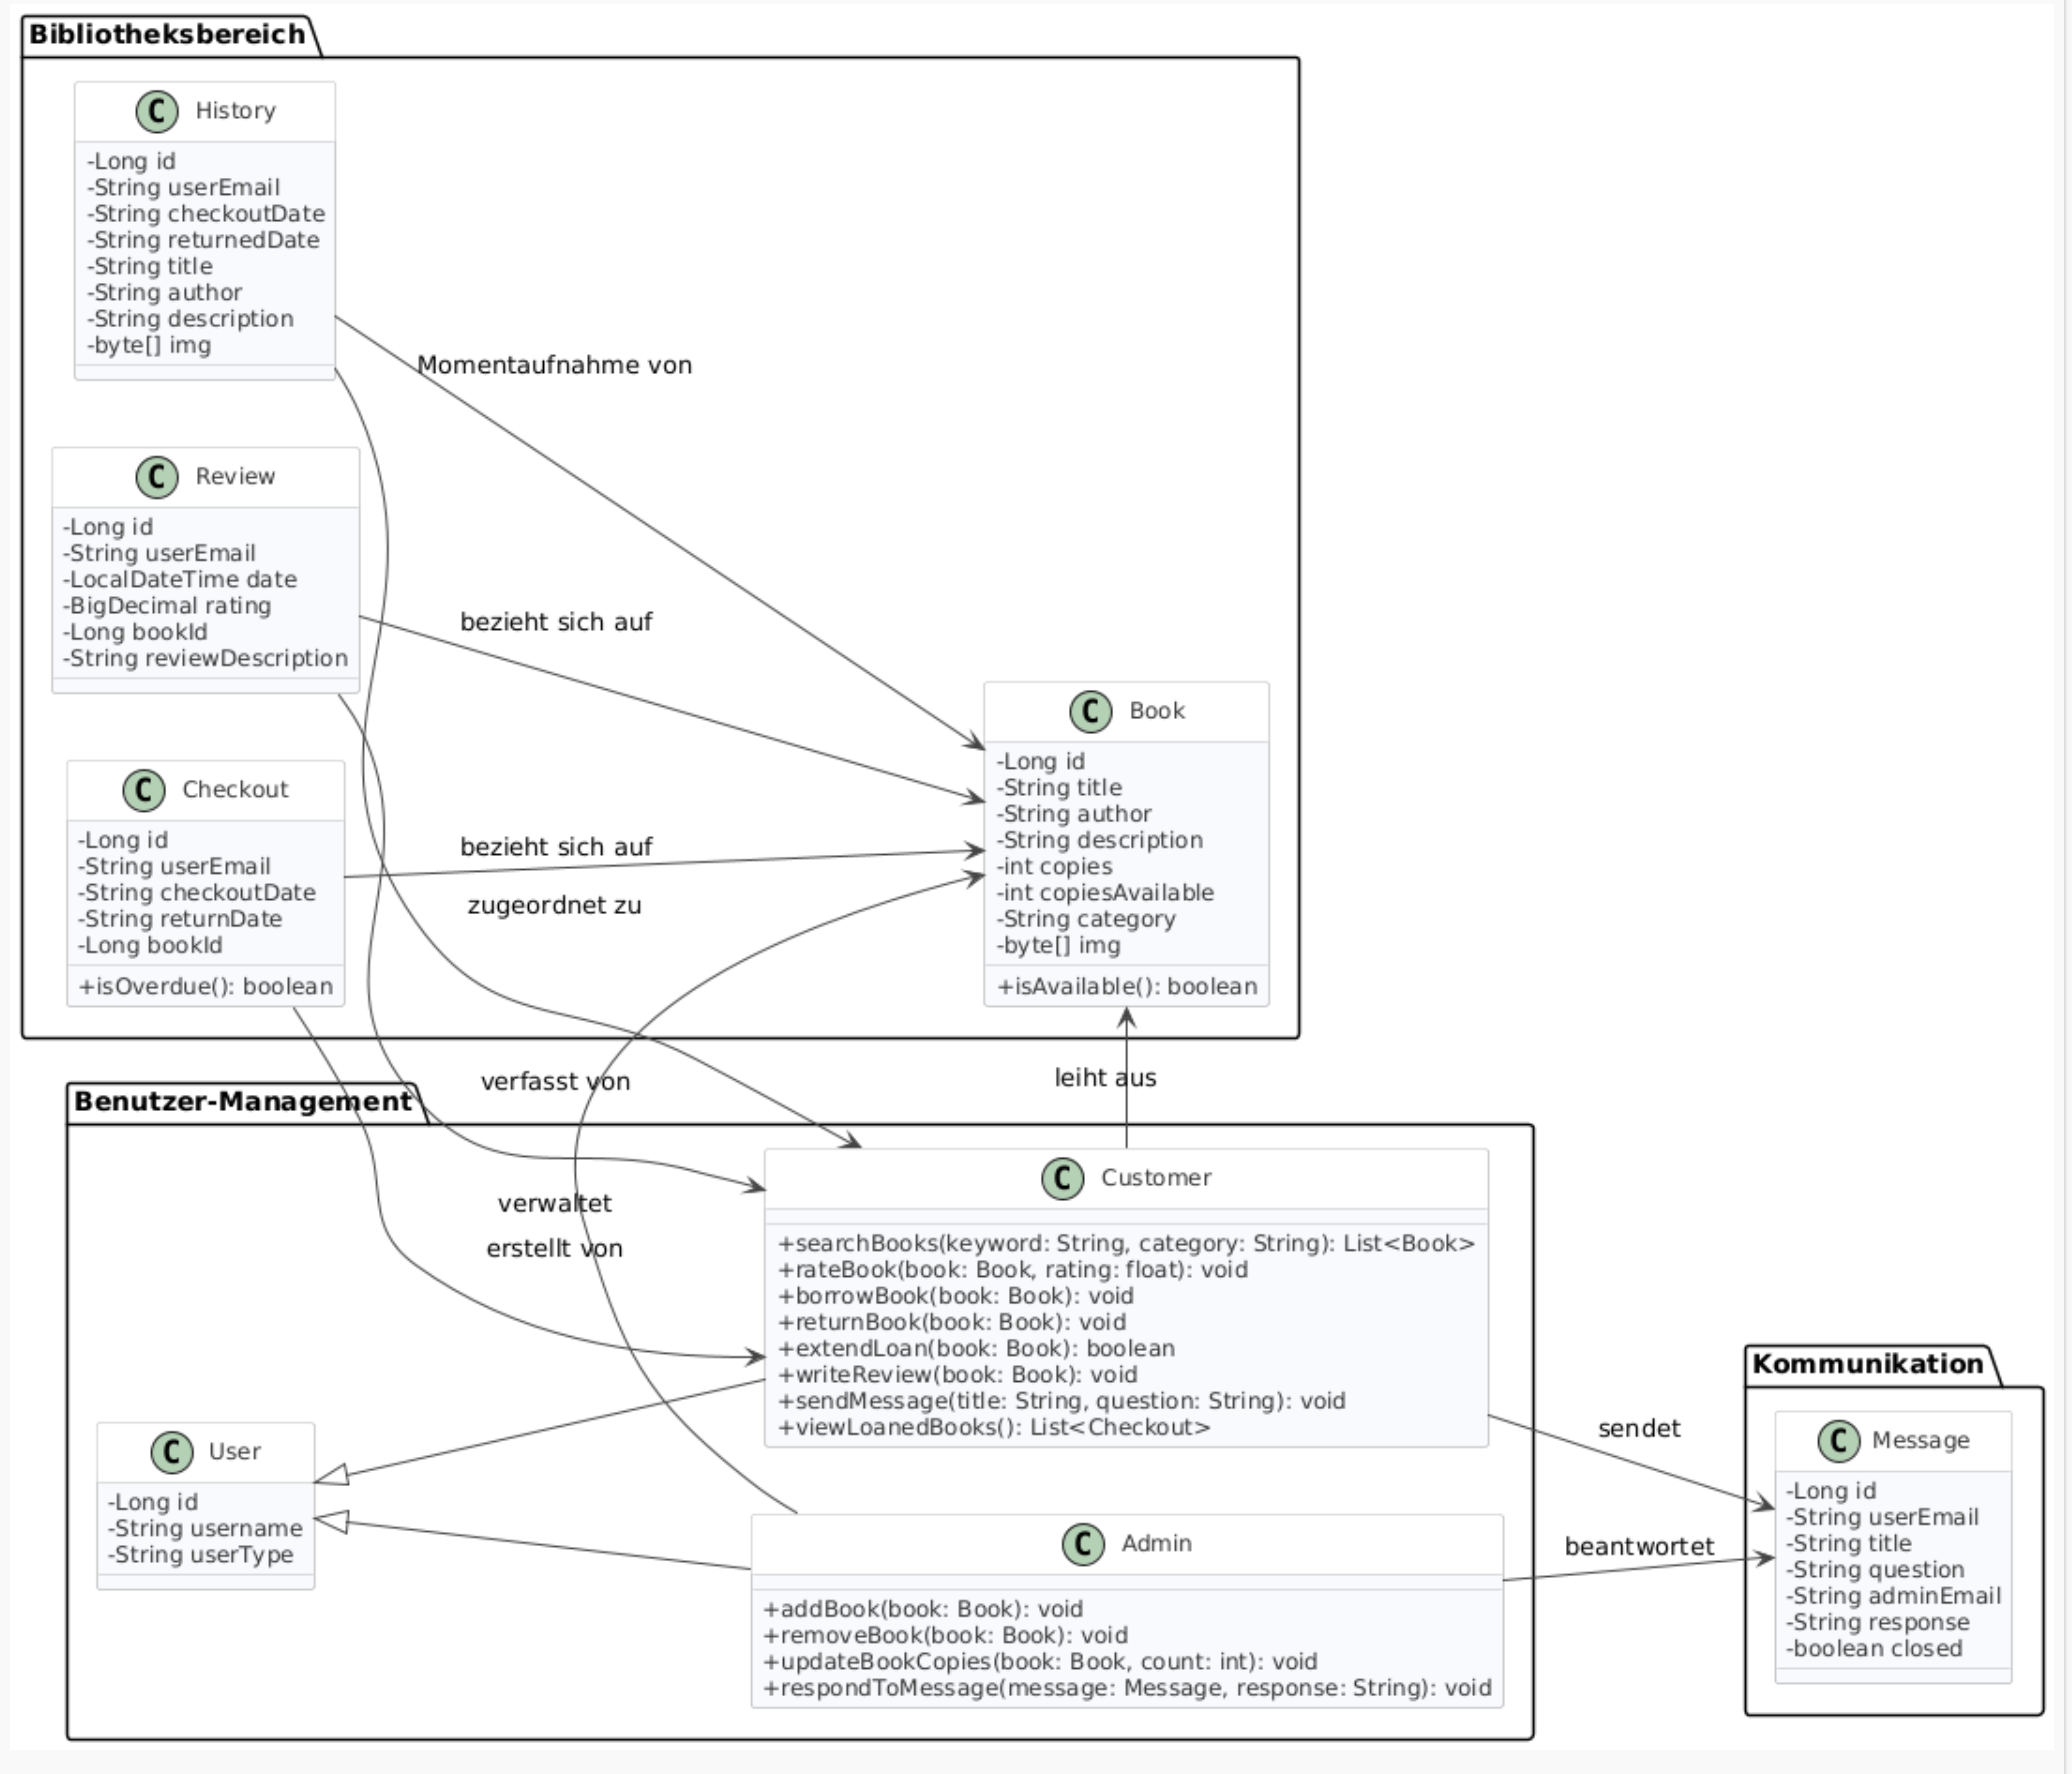
\includegraphics[width=\textwidth]{images/ClassDiagram.png}
	\caption{Klassendiagramm der Anwendung „LibraNova“}
	\label{fig:class_diagram}
\end{figure}

\subsection{Sequenzdiagramm}

Ein Sequenzdiagramm ist ein UML-Diagramm, das den zeitlichen Ablauf des Nachrichtenaustauschs zwischen Objekten in einem System darstellt. Es visualisiert, wie verschiedene Komponenten zusammenarbeiten, um bestimmte Funktionen oder Prozesse auszuführen \cite{Sequenzdiagramm:2021}.
Sequenzdiagramme sind besonders geeignet, um Kommunikationsabläufe und die Reihenfolge von Nachrichten in objektorientierten Systemen verständlich zu machen \cite[S.28]{swain2010test}.\\  \\ 
Das folgende Sequenzdiagramm  \ref{fig:Sequence-Diagram} veranschaulicht den Ablauf des Benutzer-Logins innerhalb der Anwendung. Ziel dieses Prozesses ist die sichere Authentifizierung des Benutzers sowie der Erhalt eines Tokens, um Zugriff auf geschützte Ressourcen zu ermöglichen. \\  \\
Beteiligt sind die folgenden Komponenten:
\begin{itemize}
	\item \textbf{Ressourceninhaber (Benutzer)}: startet den Anmeldevorgang und erteilt die Zustimmung zur Autorisierung.
	\item \textbf{Client-App (React)}: das Frontend, über das der Benutzer mit dem System interagiert.
	\item \textbf{Autorisierungsserver (Okta)}: authentifiziert den Benutzer und stellt einen Autorisierungscode sowie ein Access Token aus.
	\item \textbf{Ressourcenserver (Spring Boot)}: stellt geschützte Ressourcen bereit und prüft die Gültigkeit des Access Tokens.
\end{itemize}  
Der Ablauf ist wie folgt:

\begin{enumerate}
	\item Der Ressourceninhaber öffnet die React-Anwendung und startet den Login-Prozess.
	\item Die Client-Anwendung leitet den Benutzer an den Autorisierungsserver (Okta) weiter.
	\item Der Benutzer meldet sich an und stimmt der Autorisierung zu.
	\item Der Autorisierungsserver sendet einen \textit{Autorisierungscode} an die React-Anwendung.
	\item Die Client-Anwendung tauscht diesen Code beim Autorisierungsserver gegen ein \textit{Access Token} ein.
	\item Das erhaltene Token wird gespeichert (z.,B. im Speicher des Browsers).
	\item Bei einem geschützten API-Aufruf sendet die React-Anwendung das Token an den Ressourcenserver (Spring Boot).
	\item Der Ressourcenserver prüft die Gültigkeit des Tokens.
	\item Ist das Token gültig, werden die geschützten Daten zurückgegeben und dem Benutzer angezeigt.
\end{enumerate}

\begin{figure}[H]
	\centering
	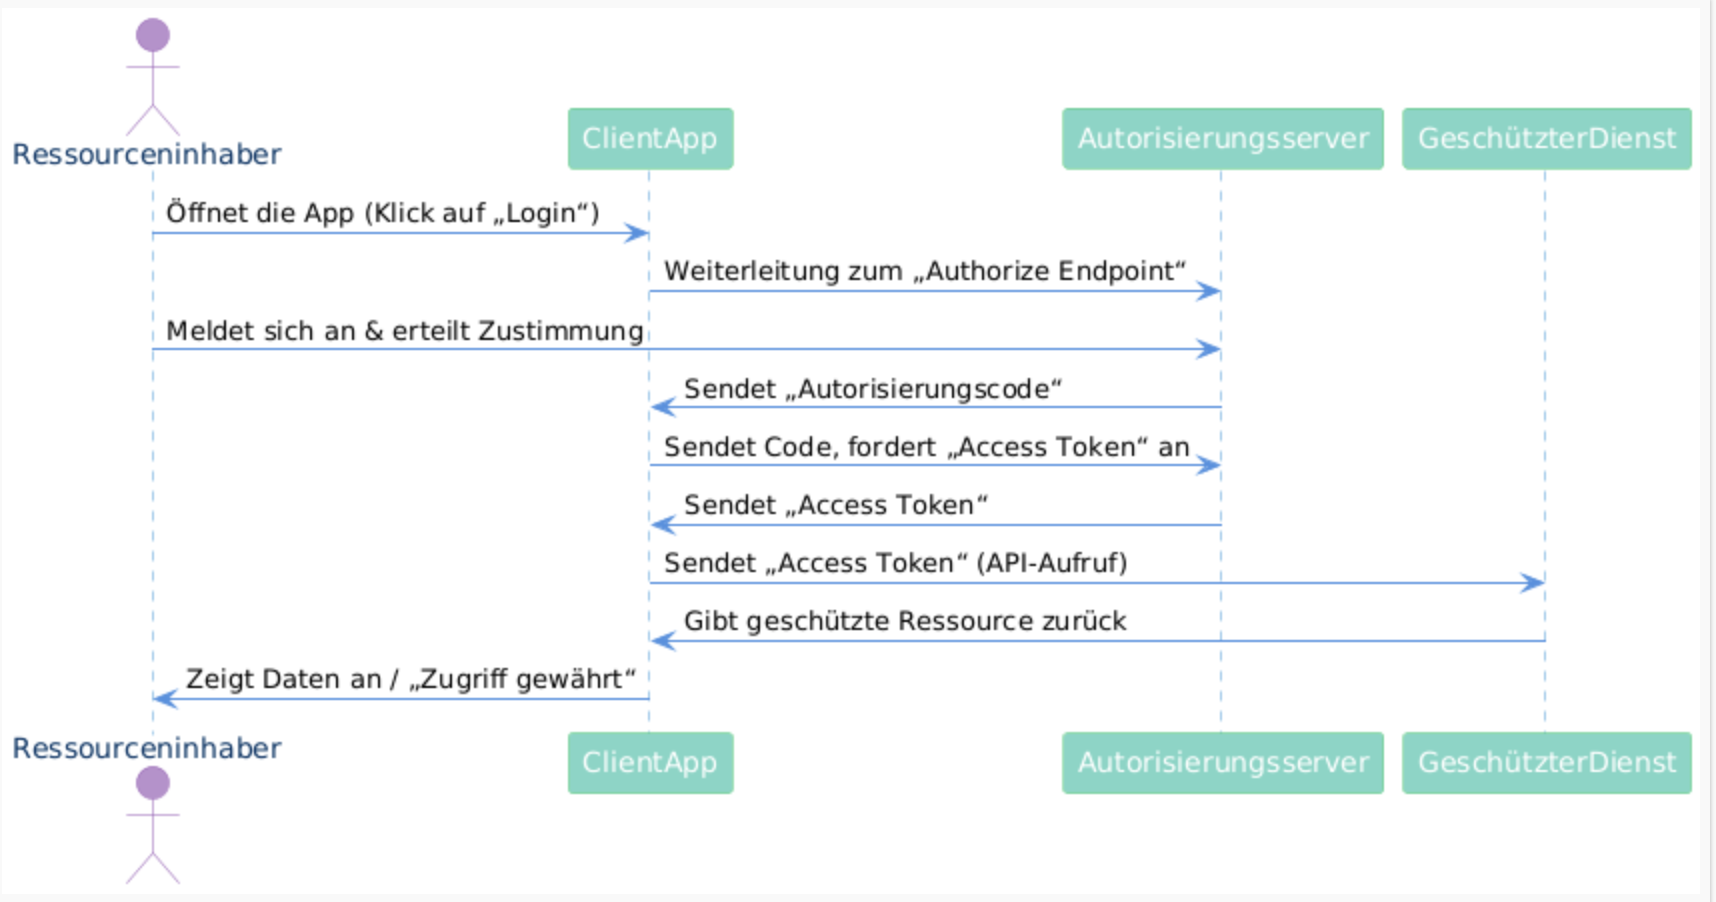
\includegraphics[width=\textwidth]{images/SequenceDiagram.jpg}
	\caption{Sequenzdiagramm des Login-Vorgangs}
	\label{fig:Sequence-Diagram} 
\end{figure}

\section{Front-End Technologien}\index{Front-End Technologien}

Dieser Abschnitt befasst sich mit den verwendeten Frontend-Technologien wie HTML, CSS, TypeScript, React und Bootstrap, die gemeinsam eine moderne, responsive und benutzerfreundliche Oberfläche für unsere Bibliotheksanwendung ermöglichen.

\subsection{HTML/CSS}\index{HTML/CSS}

HTML und CSS bilden die Grundlage für die Entwicklung und Gestaltung von Webseiten. HTML definiert die Struktur und den Inhalt der Seite, während CSS für das visuelle Erscheinungsbild zuständig ist – einschließlich Layout, Farben und Schriftarten. Gemeinsam ermöglichen sie die Erstellung ansprechender und übersichtlich strukturierter Benutzeroberflächen \cite{HTML/CSS:2024}.

\subsection{Bootstrap}\index{Bootstrap}
Bootstrap ist ein weit verbreitetes, quelloffenes Frontend-Framework zur Entwicklung responsiver und mobiler Webanwendungen. Es stellt eine Vielzahl vordefinierter CSS-Klassen sowie JavaScript-Komponenten bereit, die eine schnelle und konsistente Gestaltung von Benutzeroberflächen ermöglichen \cite{bootstrap-docs}. \\
In der vorliegenden Anwendung wurde Bootstrap eingesetzt, um das Layout flexibel zu gestalten und sicherzustellen, dass sich die Benutzeroberfläche auf verschiedenen Bildschirmgrößen (z.\,B. Desktop, Tablet, Smartphone) dynamisch anpasst. Hierfür wurden gezielt Klassen wie \texttt{container}, \texttt{row}, \texttt{col-md-*} und \texttt{d-flex} verwendet.

\subsection{Typescript}\index{Typescript}

TypeScript ist eine von Microsoft entwickelte Programmiersprache, die auf JavaScript basiert und dessen Syntax sowie Laufzeitumgebung erweitert. Im Gegensatz zu JavaScript bietet TypeScript statische Typisierung, was die frühzeitige Erkennung von Fehlern bereits während der Entwicklungsphase ermöglicht \cite{typescriptDoc}.\\ 
Für die Entwicklung der React-basierten Benutzeroberfläche wurde bewusst TypeScript anstelle von reinem JavaScript gewählt. Die Gründe dafür liegen in der besseren Code-Wartbarkeit, der verbesserten Autovervollständigung in modernen IDEs und der höheren Typsicherheit, die gerade in größeren Anwendungen wie einem Bibliotheksverwaltungssystem eine wichtige Rolle spielt \cite{typescriptBenefits}.\\ \\
In einer Anwendung zur Bibliotheksverwaltung trägt TypeScript insbesondere dazu bei, die Datenstrukturen – wie Bücher oder Ausleihvorgänge – klar zu definieren und potenzielle Typfehler bei API-Aufrufen oder Zustandsänderungen frühzeitig zu verhindern.

\subsection{React}\index{React}

React ist eine von Meta (ehemals Facebook) entwickelte JavaScript-Bibliothek zur Erstellung moderner Benutzeroberflächen. Sie basiert auf einem komponentenbasierten Architekturmodell, das eine modulare und wiederverwendbare Struktur von UI-Elementen ermöglicht. Dabei wird der Zustand der Komponenten typischerweise mit React-eigenen Mechanismen wie Hooks (useState, useEffect) verwaltet, was eine einfache und effektive Steuerung von Benutzerinteraktionen und UI-Aktualisierungen erlaubt. Besonders bekannt ist React für die Entwicklung von Single-Page Applications (SPA), bei denen Benutzerinteraktionen ohne vollständiges Neuladen der Seite verarbeitet werden, was eine schnelle und flüssige Nutzererfahrung gewährleistet \cite{react-docs, react-spa}. \\ \\
Die Kombination von React im Frontend mit Spring Boot im Backend ist weit verbreitet, da Spring Boot RESTful APIs bereitstellt, die React über HTTP-Anfragen konsumieren kann. Diese Trennung von Frontend und Backend unterstützt eine klare Architektur, fördert Skalierbarkeit und erleichtert die Wartung. Über REST APIs können dynamisch Daten wie Bücher, Benutzerinformationen oder Ausleihvorgänge in Echtzeit geladen und aktualisiert werden, was für eine Bibliotheksanwendung essenziell ist \cite{spring-rest-docs}. \\ 
React genießt große Popularität durch seine Performance, seine aktive Community sowie die umfangreiche Unterstützung durch Meta und das wachsende Ökosystem an Tools und Bibliotheken.

\section{Back-End Technologien}\index{Back-End Technologien}

In diesem Abschnitt werden die eingesetzten Back-End-Technologien analysiert, wobei der Fokus auf Spring Boot liegt – dem zentralen Framework zur Implementierung einer robusten, skalierbaren und sicheren serverseitigen Logik sowie RESTful APIs für die Anwendung LibraNova.
\subsection{Java}\index{Java}

Java ist eine weit verbreitete, objektorientierte Programmiersprache, die für ihre Plattformunabhängigkeit, Stabilität und umfangreichen Standardbibliotheken bekannt ist. Aufgrund ihrer Vielseitigkeit und Leistungsfähigkeit wird sie häufig für die Entwicklung von Back-End-Anwendungen eingesetzt. In der Bibliotheksanwendung „LibraNova“ kommt Java in der Version 17 zum Einsatz, um eine robuste, wartbare und skalierbare serverseitige Logik bereitzustellen \cite{Java:2024}.

\subsection{Spring Boot}\index{Spring Boot}

In diesem Abschnitt wird die Verwendung von Spring Boot innerhalb der Bibliotheksanwendung „LibraNova“ näher erläutert. Dabei wird aufgezeigt, welche zentralen Funktionen das Framework übernimmt, welche Module und Abhängigkeiten integriert wurden, wie Spring Boot grundsätzlich funktioniert und welche Vorteile es im Kontext dieser Anwendung bietet. Zudem wird begründet, warum sich das Projektteam bewusst für den Einsatz von Spring Boot entschieden hat.

\subsubsection{Einführung}

Spring Boot ist ein Framework, das auf dem Spring Framework aufbaut und speziell entwickelt wurde, um schnelle, effiziente und skalierbare Anwendungen zu erstellen. Es bietet eine Vielzahl von Features, die den Entwicklungsprozess beschleunigen und vereinfachen, insbesondere für Java-basierte Webanwendungen und Microservices \cite{Spring-Framework:o.J}.

\subsubsection{Gründe für die Wahl von Spring Boot}
Spring Boot wurde für die Umsetzung dieser Anwendung gewählt, da es eine Reihe bedeutender Vorteile bietet, die die Entwicklung von serverseitigen Anwendungen erheblich vereinfachen und beschleunigen. Die wichtigsten Gründe für die Entscheidung zugunsten von Spring Boot sind:
\begin{itemize}
	\item \textbf{Schneller Entwicklungsstart:} Spring Boot verfolgt einen „Opinionated“-Ansatz und stellt vorkonfigurierte Abhängigkeiten bereit, die gängige Standards und Best Practices bereits enthalten. Dadurch kann sofort mit der Entwicklung begonnen werden – ohne langwierige manuelle Konfiguration.
	
	\item \textbf{Einfache Bereitstellung:} Spring Boot-Anwendungen sind eigenständig lauffähig und benötigen keinen externen Applikationsserver. Der eingebaute Tomcat-Server ermöglicht eine unkomplizierte Ausführung der Anwendung mit einem einfachen Befehl.
	
	\item \textbf{Automatische Konfiguration:} Viele Frameworks und Bibliotheken werden automatisch erkannt und konfiguriert. Dies reduziert Boilerplate-Code und minimiert Konfigurationsaufwand.
	
	\item \textbf{Produktionsreife Funktionen:} Funktionen wie externe Konfigurationsdateien, Monitoring, Health Checks und Metriken sind bereits integriert. Dies vereinfacht nicht nur die Entwicklung, sondern auch den späteren produktiven Betrieb \cite{Spring-Framework:o.J}.
\end{itemize}

\subsubsection{Funktionsweise von Spring Boot}
Spring Boot vereinfacht die Entwicklung von Java-basierten Webanwendungen durch einen automatisierten und konventionsbasierten Startprozess. In diesem Abschnitt wird erläutert, wie ein typisches Spring-Boot-Projekt aufgebaut ist, welche Rolle die Hauptklasse spielt und wie die automatische Konfiguration sowie die Verwaltung von Anwendungseinstellungen funktioniert.

\begin{itemize}
	\item \textbf{Projektinitialisierung (Spring Initializr):} Das Projekt wurde mit dem Tool \textit{Spring Initializr} erzeugt, das eine schnelle Auswahl von Abhängigkeiten und die Generierung eines startbereiten Projekts ermöglicht.
	
	\item \textbf{Main-Klasse der Anwendung::} Die Annotation \texttt{\mbox{@SpringBootApplication}}
	 ist eine Meta-Annotation, die \texttt{@Configuration}, \texttt{@EnableAutoConfiguration} und \texttt{@ComponentScan} kombiniert. Dadurch kann Spring Boot automatisch die benötigten Konfigurationen basierend auf den eingebundenen Abhängigkeiten vornehmen und nach Komponenten, Services und Repositories suchen, um diese als Beans im Anwendungskontext zu registrieren.
	\begin{lstlisting}[language=Java, caption=Einstiegspunkt der Spring Boot Anwendung, label=lst:springboot-main, breaklines=true]
		@SpringBootApplication
		public class SpringBootLibraryApplication {
			
			public static void main(String[] args) {
				SpringApplication.run(SpringBootLibraryApplication.class, args);
			}
			
		}
	\end{lstlisting}
	
	\item \textbf{Konfigurationsdateien (\texttt{application.properties}):} Zentrale Einstellungen wie der Serverport, die Datenbankverbindung oder benutzerdefinierte Werte werden in \texttt{application.properties} definiert. Diese Datei bietet eine zentrale Steuerung der Anwendungskonfiguration.
	\begin{lstlisting}[language=, caption=Beispielhafte application.properties Datei, label=lst:application-properties, breaklines=true]
		spring.application.name=libranova
		# Datenbankkonfiguration
		spring.datasource.url=jdbc:mysql://localhost:3306/libranova_db
		spring.datasource.username=your-username
		spring.datasource.password=your-password
		spring.jpa.properties.hibernate.dialect=org.hibernate.dialect.MySQLDialect
		# REST Pfad
		spring.data.rest.base-path=/api
		# Logging 
		logging.level.org.springframework.security=DEBUG
	\end{lstlisting}
	
	
	\item \textbf{Eingebaute Webserver (Tomcat):} Spring Boot integriert standardmäßig einen eingebetteten Webserver wie Tomcat. Dadurch kann die Anwendung ohne externes Deployment direkt ausgeführt werden.
\end{itemize}

\subsubsection{Eingesetzte Abhängigkeiten (Dependencies)}\index{Spring Boot!Dependencies}
Eine Aufzählung und kurze Erklärung der wichtigsten genutzten Abhängigkeiten:
\begin{itemize}
	\item \textbf{Spring Web}: Für die Erstellung von RESTful APIs.
	\item \textbf{Spring Data JPA}: Für die Datenzugriffslogik mit JPA/Hibernate.
	\item \textbf{Spring Data REST}: Automatische Bereitstellung von REST-Endpunkten für JPA-Repositories.
	\item \textbf{Spring Boot Starter}: Vereinfacht die Projektkonfiguration durch sinnvolle Voreinstellungen.
	\item \textbf{Lombok (extern)}: Reduziert Boilerplate-Code durch automatische Generierung von Gettern, Settern usw.
\end{itemize}

\subsubsection{Spring Security}

Spring Security ist ein umfassendes und hochgradig anpassbares Framework, das speziell für die Verwaltung der Authentifizierung und Autorisierung in Java-Anwendungen entwickelt wurde. Seine Architektur ermöglicht es Entwicklern, Sicherheitsmaßnahmen zu implementieren, die auf die einzigartigen Anforderungen ihrer Anwendungen zugeschnitten sind, sodass es eine bevorzugte Wahl für Enterprise-Level-Lösungen. Das Framework bietet nicht nur wiederverwendbare Module für die Authentifizierung und Autorisierung, sondern umfasst auch Standardschutzmaßnahmen gegen gängige Web-Schwachstellen wie Cross-Site Request Forgery (CSRF) und verschiedene Exploit-Schutzmaßnahmen \cite{Spring-Security:2020}. \\ \\
Die Stärke von Spring Security liegt in seiner Flexibilität, die eine nahtlose Integration in ein breites Spektrum von Anwendungsfällen ermöglicht. Entwickler können die Funktionen leicht erweitern, um spezifische Sicherheitsanforderungen zu erfüllen, was in den dynamischen Anwendungsumgebungen von heute entscheidend ist. Dieses Anpassungspotenzial birgt jedoch auch Risiken, da unsachgemäße Konfigurationen zu erheblichen Sicherheitsschwachstellen führen können \cite{Spring-Security:2020}.\\ \\
In der Anwendung wird Spring Security verwendet, um die REST-API-Endpunkte abzusichern und den Zugriff zu kontrollieren.

\subsection{REST-API}\index{REST-API}

REST ist ein Architekturstil für die Entwicklung vernetzter Anwendungen. Er basiert auf einem zustandslosen, Client-Server- und cachefähigen Kommunikationsprotokoll, und in fast allen Fällen wird das HTTP-Protokoll verwendet. REST-APIs sind so konzipiert, dass sie einfach, leichtgewichtig und skalierbar sind, was sie zu einer beliebten Wahl für Webdienste macht \cite{REST:2024}.

\subsubsection{Einführung in REST}
Angelehnt an \cite{REST:2024} bieten REST-APIs eine Möglichkeit, über HTTP auf die Funktionalität und Daten einer Anwendung zuzugreifen. Sie folgen den Prinzipien von REST, die auf Ressourcen und deren Repräsentationen basieren. Jede Ressource wird durch eine eindeutige URI identifiziert und kann laut \cite[S.4]{Kornienko_2021} durch standardisierte HTTP-Methoden manipuliert werden:
\begin{itemize}
	\item GET: Abrufen von Ressourcen
	\item POST: Erstellen neuer Ressourcen
	\item PUT: Aktualisieren bestehender Ressourcen
	\item DELETE: Löschen von Ressourcen
\end{itemize}
REST-APIs sind aufgrund ihrer Architektur und Funktionsweise weit verbreitet und bieten eine Reihe von Vorteilen:

\begin{itemize}
	\item \textbf{Skalierbarkeit:} Durch das stateless Design können REST-APIs leicht skaliert werden. Jeder HTTP-Request enthält alle notwendigen Informationen, um ihn zu verarbeiten, ohne dass der Server den vorherigen Zustand kennen muss.
	\item \textbf{Flexibilität:} REST-APIs sind flexibel und können mit verschiedenen Datenformaten arbeiten. JSON ist das gebräuchlichste Format, da es leichtgewichtig und gut lesbar ist.
	\item \textbf{Interoperabilität:\footnote{Interoperabilität ist die Fähigkeit verschiedener Systeme oder Software, zusammenzuarbeiten und Informationen nahtlos auszutauschen\cite{wiki:listing}.}} REST-APIs nutzen standardisierte HTTP-Methoden, was ihre Interoperabilität mit verschiedenen Clients und Plattformen gewährleistet.
	\item \textbf{Leichte Integration:} REST-APIs lassen sich leicht in bestehende Systeme integrieren, da sie auf bekannten Webstandards basieren.
\end{itemize}

\subsubsection{Absicherung der REST-Endpunkte mit Spring Security}

Zur Absicherung der REST-Endpunkte in „LibraNova“ wurde das Framework \textbf{Spring Security} in Kombination mit OAuth2 und JSON Web Tokens (JWT) eingesetzt. Dabei schützt eine zentrale Sicherheitskonfiguration gezielt sensible Pfade wie \texttt{/api/books/secure/\***}, Alle übrigen Endpunkte bleiben öffentlich zugänglich. Diese Trennung zwischen geschützten und öffentlichen Routen erlaubt eine kontrollierte Zugriffskontrolle und gewährleistet gleichzeitig Offenheit für nicht sensible Daten. \\ 
Die Konfiguration erfolgt über eine \texttt{SecurityFilterChain}-Bean. Hierbei wurde die CSRF-Absicherung deaktiviert, da sie bei stateless JWT-Authentifizierung überflüssig ist. Gleichzeitig wird eine OAuth2-Resource-Server-Konfiguration mit JWT-Validierung verwendet. Die Einrichtung einer \texttt{ContentNegotiationStrategy} unterstützt eine saubere Inhaltsaushandlung zwischen Client und Server. Die Integration der \texttt{Okta.configureResourceServer401ResponseBody(http)}-Methode verbessert zudem die Fehlerbehandlung bei unautorisierten Zugriffen.

\begin{lstlisting}[language=Java, caption={Spring Security-Konfiguration}]
	http
	.csrf(csrf -> csrf.disable())
	.authorizeHttpRequests(configurer -> configurer
	.requestMatchers("/api/books/secure/**", 
	"/api/reviews/secure/**", 
	"/api/messages/secure/**", 
	"/api/admin/secure/**").authenticated()
	.anyRequest().permitAll())
	.oauth2ResourceServer(oauth2 -> oauth2.jwt())
	.cors(cors -> cors.configurationSource(corsConfigurationSource()));
\end{lstlisting}
Durch diese Konfiguration wird sichergestellt, dass nur authentifizierte Nutzer mit gültigem JWT-Token auf geschützte Ressourcen zugreifen können, während gleichzeitig der Zugriff auf öffentliche Inhalte uneingeschränkt möglich bleibt.

\subsubsection{CORS-Konfiguration und Einschränkung von HTTP-Methoden}

Zur zusätzlichen Absicherung des Backends wurden zwei Maßnahmen umgesetzt: Erstens wurde eine \textbf{CORS-Konfiguration} implementiert, die ausschließlich Anfragen vom React-Frontend (\texttt{https://localhost:3000}) erlaubt. Zweitens wurden mithilfe von \texttt{RepositoryRestConfigurer} bestimmte HTTP-Methoden wie \texttt{POST}, \texttt{PUT}, \texttt{PATCH} und \texttt{DELETE} auf ausgewählten Entitäten deaktiviert, um ungewollte Änderungen über Spring Data REST zu verhindern.

\begin{lstlisting}[language=Java, caption={CORS und HTTP-Methodenbeschränkung}]
	config.exposeIdsFor(Book.class, Review.class, Message.class);
	
	HttpMethod[] unsupported = {POST, PUT, PATCH, DELETE};
	restrictHttpMethods(Book.class, config, unsupported);
	
	corsRegistry.addMapping(config.getBasePath() + "/**")
	.allowedOrigins("https://localhost:3000");
\end{lstlisting}
Diese Konfiguration trägt maßgeblich zur Sicherheit und Stabilität der Anwendung bei, indem sie sowohl die erlaubten Ursprünge als auch die zulässigen Zugriffsarten explizit definiert.

\subsection{HTTPS und SSL/TLS}
In diesem Abschnitt wird erläutert, wie die Anwendung durch die Integration von HTTPS und SSL/TLS eine sichere und verschlüsselte Kommunikation zwischen Client und Server gewährleistet.

\subsubsection{Grundlagen von HTTPS und SSL/TLS}

HTTPS ist die verschlüsselte Version von HTTP und schützt die Kommunikation zwischen Client und Server \cite{HTTPS:2024}. Dabei kommen die Protokolle SSL/TLS zum Einsatz, wobei TLS als moderner und sicherer Standard gilt \cite{SSL/TLS:2023}. Sie gewährleisten:

\begin{itemize}
	\item \textbf{Verschlüsselung:} Schutz der übertragenen Daten vor unbefugtem Zugriff.
	\item \textbf{Authentifizierung:} Sicherstellung, dass der Server legitim ist.
	\item \textbf{Datenintegrität:} Verhinderung der Manipulation von Daten während der Übertragung.
\end{itemize}

\subsubsection{SSL-Konfiguration im Backend}

Zur Absicherung des Datenverkehrs wurde in der Anwendung eine HTTPS-Konfiguration implementiert, bei der der Server auf Port \texttt{8443} HTTPS-Anfragen entgegennimmt (siehe \ref{HTTPS-Config}). Dafür wurde SSL/TLS aktiviert, um eine verschlüsselte Kommunikation zwischen Client und Server zu gewährleisten. \\
Die Verschlüsselung basiert auf einem selbstsignierten SSL-Zertifikat, das mit dem folgenden Befehl generiert wurde:
\begin{lstlisting}[language=bash, caption={Generierung eines SSL-Zertifikats}, breaklines=true]
	keytool -genkeypair -alias libranova \
	-keystore src/main/resources/libranova-keystore.p12 \
	-keypass secret -storepass secret -storeType PKCS12 \
	-keyalg RSA -keysize 2048 -validity 365 \
	-dname "C=DE, ST=Rhineland-Palatinate, L=Trier, O=libranova, OU=Studies Backend, CN=localhost" \
	-ext "SAN=dns:localhost"
\end{lstlisting}
Dabei wurde eine Keystore-Datei im \texttt{PKCS12}-Format (\texttt{libranova-keystore.p12}) erstellt, in der das Zertifikat unter dem Alias \texttt{libranova} gespeichert ist. Diese Datei wird in der \texttt{application.properties} wie folgt eingebunden:

\begin{lstlisting}[language=, label=HTTPS-Config, caption={HTTPS- und SSL-Konfiguration}]
	# HTTPS settings
	server.port=8443
	server.ssl.enabled=true
	server.ssl.key-alias=libranova
	server.ssl.key-store=classpath:libranova-keystore.p12
	server.ssl.key-store-password=secret
	server.ssl.key-store-type=PKCS12
\end{lstlisting}
Durch diese Konfiguration wird sichergestellt, dass alle übermittelten Daten verschlüsselt und vor unbefugtem Zugriff geschützt sind. Die Anwendung erfüllt damit grundlegende Sicherheitsanforderungen moderner Webanwendungen.


\subsubsection{SSL-Konfiguration im Frontend}

Auch im Frontend wurde eine lokale HTTPS-Verbindung eingerichtet, um eine verschlüsselte Kommunikation mit dem Backend zu ermöglichen. Dazu wurde mithilfe von OpenSSL ein selbstsigniertes Zertifikat erstellt:

\begin{lstlisting}[language=bash, caption={Generierung eines Frontend-Zertifikats}]
	openssl req -x509 \
	-out ssl-localhost-libranova/localhost.crt \
	-keyout ssl-localhost-libranova/localhost.key \
	-newkey rsa:2048 -nodes -sha256 -days 365 \
	-config localhost.conf
\end{lstlisting}
Dieses Kommando erzeugte zwei Dateien:
\begin{itemize}
	\item \texttt{localhost.crt} – das Zertifikat
	\item \texttt{localhost.key} – der zugehörige private Schlüssel
\end{itemize}
In der \texttt{.env}-Datei wurden diese Dateien anschließend referenziert, um die React-Entwicklungsumgebung über HTTPS zu betreiben:

\begin{lstlisting}[language=bash, caption={.env Konfiguration für HTTPS und API-Zugriff}]
	SSL_CRT_FILE=ssl-localhost-libranova/localhost.crt
	SSL_KEY_FILE=ssl-localhost-libranova/localhost.key
	REACT_APP_API_URL='https://localhost:8443/api'
\end{lstlisting}
Die Konfigurationsdatei \texttt{localhost.conf} enthielt die benötigten Informationen für das Zertifikat (wie Standort und Common Name), um den Generierungsprozess zu automatisieren:

\begin{lstlisting}[caption={localhost.conf}]
	[req]
	prompt = no
	distinguished_name = dn
	
	[dn]
	C = DE
	ST = Rhineland-Palatinate
	L = Trier
	O = Libranova
	OU = Studies
	CN = localhost
\end{lstlisting}
Diese Konfiguration ermöglicht eine sichere Verbindung zwischen Frontend und Backend während der lokalen Entwicklung. \\ \\
Die HTTPS-Implementierung mit SSL/TLS gewährleistet die Einhaltung von Sicherheitsstandards und schützt sensible Nutzerdaten zuverlässig.



\subsection{Stripe API}

\subsubsection{Überblick}

\subsubsection{Hauptmerkmale der Stripe API}

\subsubsection{Stripe API Integration für nahtlose Zahlungsabwicklung}

\section{Datenbankstruktur}\index{Datenbankstruktur}
In diesem Abschnitt wird die Datenbankstruktur der Webanwendung untersucht, um ein umfassendes Verständnis für die Organisation, den Zugriff und die Verwaltung der Daten zu vermitteln. Der Schwerpunkt liegt auf dem relationalen Datenbankmodell und den spezifischen Technologien und Frameworks, die zur Handhabung der Datenpersistenz und der Transaktionen verwendet werden. Dabei wird MySQL als das gewählte Datenbanksystem zusammen mit Spring Data JPA für eine nahtlose Dateninteraktion untersucht. In den folgenden Unterabschnitten werden diese Aspekte im Detail behandelt, wobei relationale Datenbanken, die Auswahl von MySQL, Datenpersistenz und Transaktionsmanagement sowie die Integration von MySQL mit Spring Boot behandelt werden.
\subsection{Übersicht über relationale Datenbanken und Auswahl von MySQL}
Relationale Datenbanken speichern Daten in Tabellen und nutzen Schlüssel zur Definition von Beziehungen. Für ein Bibliotheksverwaltungssystem eignet sich dieses Modell gut, da es komplexe Verknüpfungen zwischen Entitäten wie Büchern und Ausleihvorgängen unterstützt. MySQL wurde gewählt, da es strukturierte Daten zuverlässig verarbeitet, komplexe Abfragen effizient unterstützt und sich stabil mit Spring Boot integrieren lässt \cite{IBM:o.J}.

\subsection{Entitäten und Datenbankabbildung mit Spring Data JPA}
\label{sec:entity_mapping}

Zur Modellierung der Datenstruktur der Bibliotheksanwendung kommen mehrere Entitäten zum Einsatz, die jeweils einer Tabelle in der zugrundeliegenden relationalen Datenbank entsprechen. Die Abbildung erfolgt über JPA-Annotationen wie \texttt{@Entity}, \texttt{@Id} und \texttt{@Column}. Dadurch wird eine klare, objektorientierte Repräsentation der Daten erreicht. \\ \\
Zu den zentralen Entitäten gehören:

\begin{itemize}
	\item \textbf{Book}: Enthält grundlegende Informationen über verfügbare Bücher, wie Titel, Autor, Kategorie, verfügbare Exemplare und Beschreibung.
	\item \textbf{Checkout}: Repräsentiert die Ausleihvorgänge, wobei jedem Eintrag eine Benutzer-E-Mail, ein Buch und Ausleih- sowie Rückgabedatum zugeordnet sind.
	\item \textbf{History}: Dokumentiert abgeschlossene Ausleihvorgänge und speichert relevante Buch- und Benutzerdaten.
	\item \textbf{Review}: Ermöglicht es Nutzern, Bewertungen zu Büchern zu hinterlassen. Enthält Angaben wie Bewertung, Rezensionstext und das Erstellungsdatum.
	\item \textbf{Message}: Dient der Kommunikation zwischen Nutzern und Administratoren, insbesondere für Supportanfragen.
\end{itemize}
Die Verwaltung der Entitäten erfolgt über Spring Data JPA. Interfaces wie \texttt{JpaRepository} ermöglichen CRUD-Operationen und komplexe Abfragen ohne eigenen SQL-Code. Das \texttt{BookRepository}  (siehe \ref{lst:bookrepo}) bietet Methoden mittels benutzerdefinierter Queries. \\ \\
\begin{lstlisting}[language=Java, caption={Ausschnitt aus dem BookRepository}, label={lst:bookrepo}, breaklines=true]
	public interface BookRepository extends JpaRepository<Book, Long> {
		Page<Book> findByTitleContainingIgnoreCase(@RequestParam("title") String title, Pageable pageable);
		
		Page<Book> findByCategory(@RequestParam("category") String category, Pageable pageable);
		
		@Query("SELECT b FROM Book b WHERE b.id IN :book_ids")
		List<Book> findBooksByBookIds(@Param("book_ids") List<Long> bookId);
	}
\end{lstlisting}
Diese strukturierte und erweiterbare Modellierung bildet das Fundament für die Datenpersistenz und stellt sicher, dass alle Anwendungskomponenten konsistent mit der Datenbank interagieren.

\subsection{MySQL-Workbench und SQL}
MySQL Workbench dient als Werkzeug für den Entwurf und die Verwaltung der Datenbank, während SQL als Sprache zur Erstellung von Abfragen und zur Datenbankverwaltung eingesetzt wird. \\ \\
Mit MySQL Workbench wurde das Datenbankschema visualisiert, was eine intuitive Gestaltung und Pflege der Datenbankstrukturen ermöglicht. So konnten Tabellen, Beziehungen und Indizes einfach erstellt und angepasst werden. Zusätzlich kam SQL zum Einsatz, um Abfragen für Tests durchzuführen sowie Aufgaben wie Datenmanipulation und Schemaänderungen vorzunehmen \cite{mySQL:o.J}. 

\section{Authentifizierungs- und Autorisierungsprotokolle}\index{Authentifizierungs- und Autorisierungsprotokolle}

Sichere Benutzerverwaltung und Zugriffskontrolle sind für Webanwendungen entscheidend. Technologien wie Okta, JWT, OAuth2 und OpenID Connect sorgen für standardisierte Authentifizierung und Autorisierung. Im Folgenden wird ihre Nutzung in der Anwendung beschrieben.

\subsection{Okta}
Okta ist ein cloudbasierter Identitätsdienst, der sicheren Zugriff auf Anwendungen und Geräte ermöglicht. Es bietet Single Sign-On (SSO), Multi-Faktor-Authentifizierung (MFA) und Integration mit lokalen Verzeichnissen wie Active Directory. Okta erleichtert das Identitäts- und Zugriffsmanagement über verschiedene Systeme hinweg \cite{Okta:o.J}. \\ \\
In dieser Anwendung dient Okta als externer Identitätsanbieter zur sicheren und effizienten Verwaltung von Authentifizierung und Autorisierung. Das Frontend in React nutzt das Okta Sign-In Widget und SDK, um Benutzeranmeldungen, Sitzungsmanagement und Token-Verwaltung abzuwickeln. Im Backend validiert die Spring Boot-Anwendung diese Tokens mithilfe des Okta Spring Boot Starters, um sicherzustellen, dass nur authentifizierte und autorisierte Nutzer auf geschützte API-Endpunkte zugreifen können. \\ \\
Der Hauptzweck der Okta-Integration bestand darin, die Komplexität der sicheren Nutzerverwaltung auszulagern – einschließlich Passwortverwaltung, Token-Ausgabe und rollenbasierter Zugriffskontrolle. So konnte ein standardisierter und effizienter Authentifizierungsprozess umgesetzt werden, der unterschiedliche Benutzerrollen (z. B. Admins und normale Nutzer) unterstützt und die Berechtigungen direkt in Okta verwaltet. Insgesamt verbessert die Einbindung von Okta die Sicherheit, Skalierbarkeit und Wartbarkeit des Authentifizierungsflusses, ohne das Rad neu erfinden zu müssen.

\subsection{JWT}

JWT ist ein offener Standard zur sicheren Übertragung von Informationen als signiertes JSON-Objekt. Es wird hauptsächlich für die Autorisierung genutzt, indem es nach der Anmeldung den Zugriff auf geschützte Ressourcen ermöglicht. Außerdem gewährleistet JWT die Integrität und Authentizität der übertragenen Daten. \cite{JWT:o.J}.  \\ \\
In der Anwendung werden von Okta ausgestellte JWTs verwendet, um API-Endpunkte zu sichern. Spring Security ist als OAuth2-Resource-Server konfiguriert, der die JWTs validiert. Die Tokens enthalten Benutzer-Claims wie den benutzerdefinierten „userType“, der in den Controllern ausgelesen wird, um rollenbasierte Zugriffssteuerung umzusetzen. So wird sichergestellt, dass z. B. nur Admins bestimmte Aktionen durchführen können. Dieses Setup gewährleistet eine sichere, tokenbasierte Authentifizierung und feingranulare Autorisierung im Backend.


\subsection{OAuth2}
OAuth 2.0 ist ein Sicherheitsstandard, der Drittanbieteranwendungen ermöglicht, im Namen von Nutzern auf Ressourcen zuzugreifen, ohne deren Anmeldedaten preiszugeben. Es basiert auf dem Austausch von Zugriffstokens, was die Sicherheit erhöht \cite{OAuth2:2023}.  \\ \\
In der Anwendung wird OAuth 2.0 zusammen mit Okta genutzt, um JWTs auszustellen und zu validieren. Diese Tokens autorisieren den Zugriff auf geschützte Backend-Ressourcen, wodurch eine sichere und rollenbasierte Zugriffskontrolle gewährleistet wird.

\subsection{OpenID Connect}
OpenID Connect ist ein Authentifizierungsprotokoll, das auf OAuth 2.0 basiert und die sichere Überprüfung der Benutzeridentität ermöglicht. Es liefert standardisierte Nutzerinformationen und unterstützt eine einfache Integration in verschiedene Anwendungen \cite{OpenId:o.J}. \\ \\
In der Anwendung wird OpenID Connect über Okta genutzt, um eine zuverlässige und interoperable Benutzeranmeldung sicherzustellen. Dabei stellt OpenID Connect die Identitätsinformationen als ID-Token bereit, die vom Backend zur Authentifizierung und Autorisierung der Benutzer überprüft werden. So kann die Anwendung Benutzerrollen sicher handhaben und den Zugriff auf geschützte Ressourcen kontrollieren.


\section{Entwicklungsumgebung und Versionskontrolle}\index{Entwicklungsumgebung und Versionskontrolle}
In diesem Abschnitt werden die integrierten Entwicklungsumgebungen (IDEs) und Versionskontrollsysteme beschrieben, die im Rahmen des Projekts eingesetzt wurden. Er bietet einen Überblick über die für die Entwicklung ausgewählten IDEs und die Versionskontrollwerkzeuge, die zur effektiven Verwaltung von Codeänderungen eingesetzt wurden.
\subsection{Entwicklungsumgebung}
Für die Entwicklung des Backends wurde IntelliJ IDEA Community Edition verwendet, eine kostenlose und weit verbreitete IDE, die besonders gut für Spring Boot Projekte geeignet ist. Für das Frontend kam Visual Studio Code zum Einsatz, ebenfalls eine kostenlose und sehr beliebte Entwicklungsumgebung, die sich durch ihre Flexibilität und umfangreiche Erweiterungen auszeichnet. Beide Tools gehören zu den meistgenutzten in der Softwareentwicklung und haben die effiziente Umsetzung der Anwendung unterstützt.


\subsection{Versionskontrollsysteme: Git und GitHub}

In diesem Unterabschnitt werden die im Projekt eingesetzten Versionskontrollsysteme Git und GitHub beschrieben. Git ist ein kostenloses, verteiltes Versionskontrollsystem, das durch schnelle Performance, effizientes Verzweigungsmanagement und flexible Arbeitsabläufe überzeugt. Es ermöglicht eine einfache Verwaltung von Projekten jeder Größe und fördert die parallele Entwicklung durch lokale Branches \cite{git-scmr:o.J}.\\ \\
GitHub ergänzt Git als cloudbasierte Plattform für das Speichern, Teilen und die Zusammenarbeit an Code. Es erleichtert das Verfolgen von Änderungen, die Überprüfung durch andere Entwickler sowie die koordinierte Zusammenarbeit, ohne unbeabsichtigte Auswirkungen auf den Hauptcode zu riskieren \cite{github:o.J}. Beide Tools haben wesentlich zur effizienten Codeverwaltung und Versionskontrolle im Verlauf des Projekts beigetragen.

\section{Testen und Qualitätssicherung}\index{Testen und Qualitätssicherung}

\subsection{Backend-Tests}
\begin{itemize}
	\item Unit-Tests mit JUnit
	\item Mocking und Dependency Injection mit Mockito
	\item Integrationstests mit Spring Test
\end{itemize}

\subsection{Frontend-Tests}
\begin{itemize}
	\item Komponenten- und UI-Tests mit React Testing Library und Jest
\end{itemize}

\subsection{API-Tests}
\begin{itemize}
	\item Manuelle und automatisierte API-Tests mit Postman
\end{itemize}













